\section{Phân tích tổng quan các hệ thống có liên quan trên thị trường}

\subsection{Hệ thống Quản lý và Tra cứu Tài nguyên Thư viện – Đại học Bách Khoa TP.HCM}

Hệ thống quản lý và tra cứu tài nguyên thư viện của Trường Đại học Bách Khoa – ĐHQG TP.HCM hiện đang được vận hành thông qua hai cổng thành phần độc lập nhưng bổ trợ lẫn nhau: Cổng thông tin Thư viện chính thức (tại địa chỉ \url{https://lib.hcmut.edu.vn/}) và Hệ thống Tra cứu công cộng trực tuyến (OPAC tại địa chỉ \url{https://opac.lib.hcmut.edu.vn/}). Sự kết hợp này nhằm mục đích quản lý và phục vụ song song hai nguồn tài nguyên cốt lõi của nhà trường: tài liệu in ấn truyền thống và kho tài liệu nội sinh đặc thù.

Đối với cổng thông tin thư viện chính (\url{lib.hcmut.edu.vn}), hệ thống đóng vai trò là trung tâm quản lý và giới thiệu toàn bộ nguồn tài liệu in bao gồm sách giáo trình, tài liệu tham khảo, tạp chí chuyên ngành thuộc nhiều lĩnh vực đang được lưu trữ vật lý tại các kho sách của trường (như Kho sách mượn tòa nhà B2, Kho sách tham khảo tòa nhà B4 tại cơ sở Lý Thường Kiệt, và Thư viện tại Cơ sở Dĩ An). Người dùng tại giao diện này chủ yếu tiếp cận các thông tin mang tính thông báo, quy chế mượn trả, hoặc sử dụng thanh tìm kiếm nhanh để xác định sự tồn tại và số lượng khả dụng của các đầu sách in trong kho thực tế.

\begin{figure}[H]
    \centering
     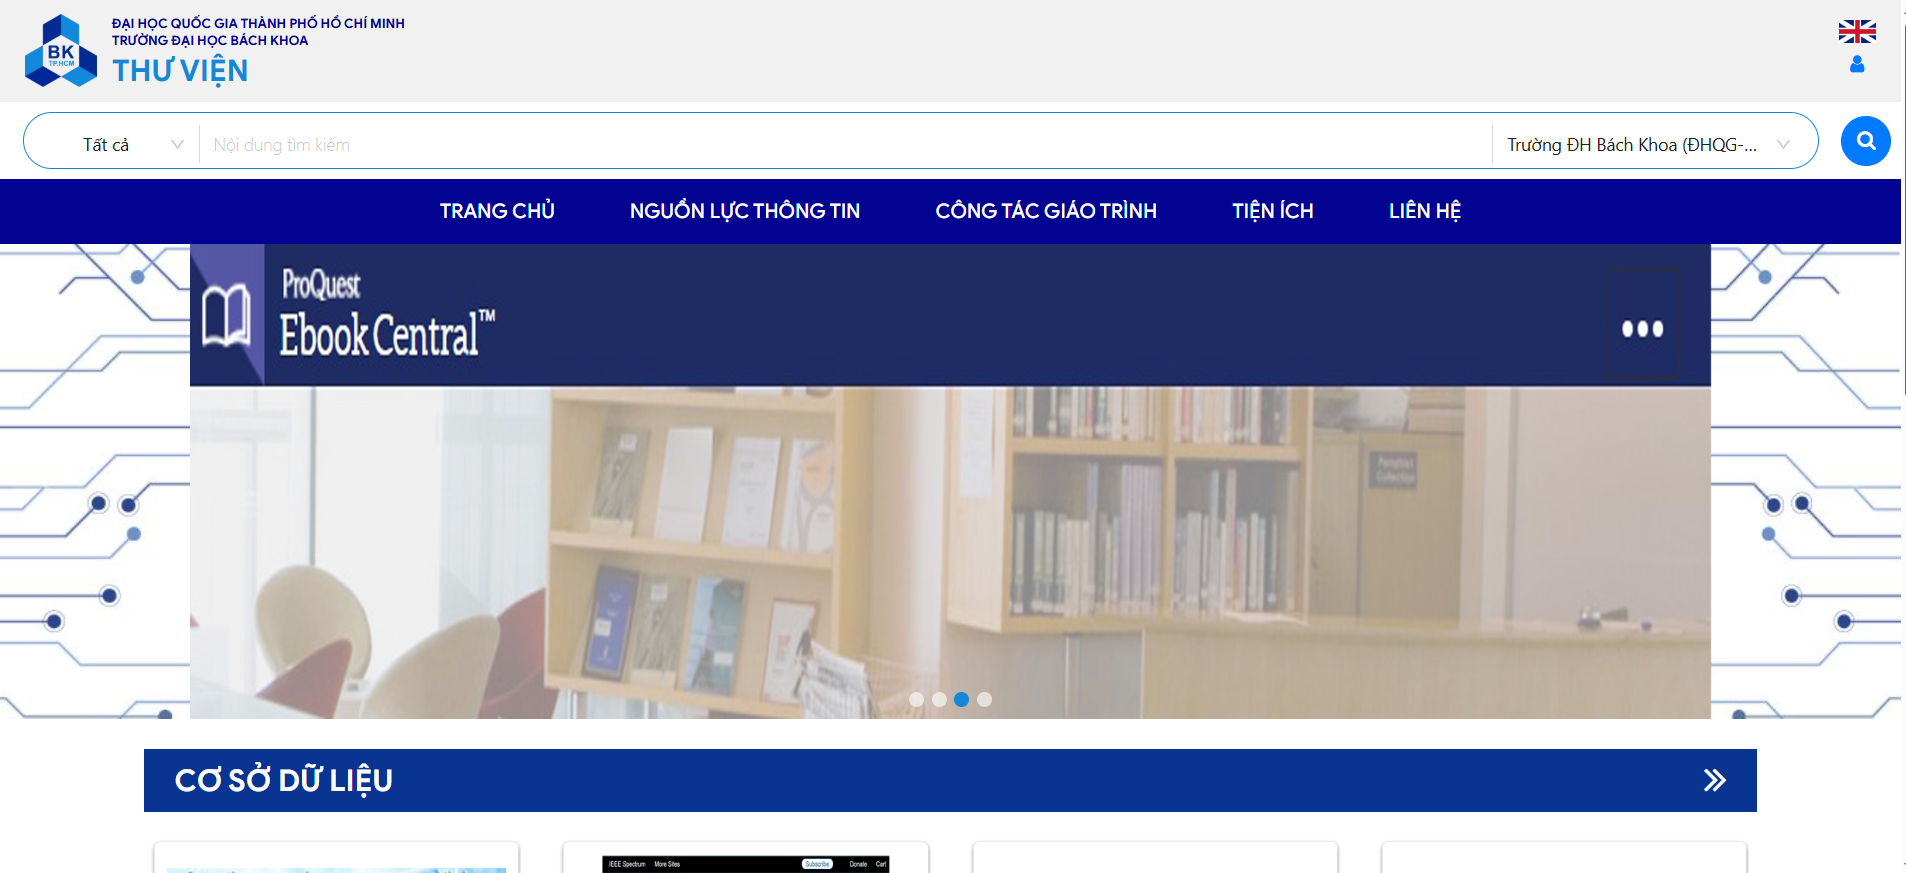
\includegraphics[width=0.8\linewidth]{Images/lib_hcmut_homepage.png} 
     \vspace{10pt}
    \caption{Giao diện trang chủ Cổng thông tin Thư viện lib.hcmut.edu.vn và danh mục tài liệu in}
    \label{fig:lib_hcmut_homepage}
\end{figure}

Song song đó, để phục vụ nhu cầu khai thác sâu các công trình nghiên cứu học thuật, nhà trường triển khai cổng OPAC (\url{opac.lib.hcmut.edu.vn}), đóng vai trò là cổng tra cứu chuyên biệt dành cho tài liệu nội sinh. Đây là nơi lưu trữ và số hóa toàn bộ các tài sản trí tuệ được sản sinh từ chính nội bộ nhà trường, bao gồm: luận văn tốt nghiệp của sinh viên, luận án thạc sĩ, tiến sĩ của học viên cao học, cùng các đề tài nghiên cứu khoa học các cấp của cán bộ, giảng viên. Giao diện OPAC cung cấp các công cụ lọc siêu dữ liệu (metadata) chuyên sâu theo Tác giả, Người hướng dẫn, Năm bảo vệ, hoặc Chuyên ngành đào tạo.

Hệ thống OPAC cũng được tích hợp sâu với phương thức xác thực tập trung của nhà trường (Cổng đăng nhập SSO/BKPay). Khi đăng nhập thành công vào phân hệ "Tài khoản cá nhân", bạn đọc có thể chủ động quản lý các tác vụ lưu thông như danh sách các tài liệu đang mượn, lịch sử các lần mượn trước đó, theo dõi các khoản phí phạt phát sinh do quá hạn, đăng ký gia hạn thời gian mượn đối với các sách sắp đến hạn, hoặc thực hiện đặt giữ chỗ trước đối với những tài liệu hiện đang được mượn hết trong kho.

\begin{figure}[H]
    \centering
    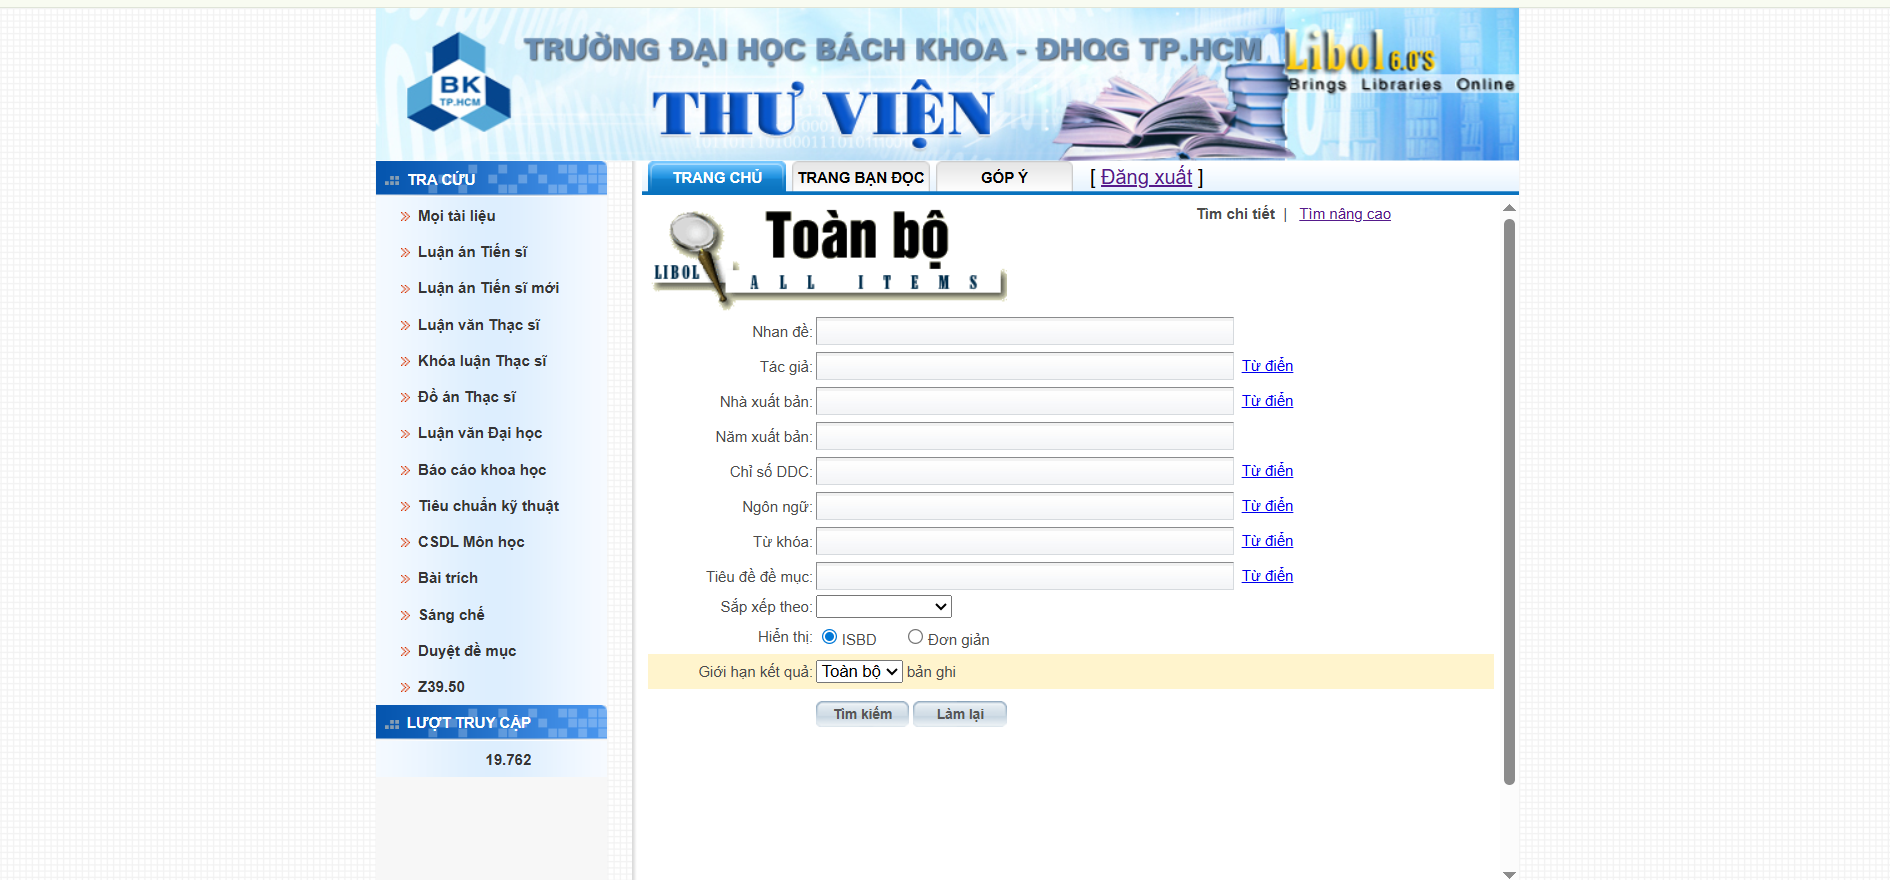
\includegraphics[width=0.8\linewidth]{Images/opac.lib.hcmut.edu.vn.png} 
     \vspace{10pt}
    \caption{Giao diện Tra cứu Tài liệu Nội sinh và phân hệ Đăng nhập tài khoản trên cổng OPAC}
    \label{fig:opac_hcmut_search}
\end{figure}

Mặc dù cả hai cổng đang đáp ứng tốt các nghiệp vụ cơ bản, tuy nhiên việc phân mảnh dữ liệu giữa tài liệu in và tài tài liệu số/nội sinh đang tạo ra rào cản nhất định trong trải nghiệm của sinh viên. Đây chính là động lực để nhóm nghiên cứu hướng tới việc xây dựng một hệ thống quản lý thư viện hiện đại, hợp nhất dữ liệu và tối ưu hóa quy trình thông qua các giải pháp công nghệ mới.

\subsubsection{Điểm mạnh}
\begin{itemize}
    \item Giao diện chuyên biệt cho tài liệu nội sinh giúp tối ưu hóa việc tìm kiếm các trường dữ liệu đặc thù.
    \item Luồng nghiệp vụ mượn trả và đặt giữ chỗ trực tuyến tương thích hoàn toàn với quy chế vận hành thực tế.
    \item Cơ chế xác thực một lần (SSO) giúp đồng bộ dữ liệu tài khoản bạn đọc và bảo mật tài nguyên số.
\end{itemize}

\subsubsection{Điểm yếu}
\begin{itemize}
    \item Việc duy trì hai hệ thống độc lập bắt buộc bạn đọc phải thực hiện tra cứu nhiều lần trên các tên miền khác nhau.
    \item Cơ chế tra cứu phụ thuộc hoàn toàn vào từ khóa khớp chính xác, chưa xử lý tốt ngôn ngữ tự nhiên.
    \item Hệ thống mang tính tĩnh, chưa có tính năng gợi ý tự động và thiếu vắng công cụ trợ lý ảo hỗ trợ bạn đọc 24/7.
    \item Giao diện tra cứu chuyên sâu chưa tối ưu tốt cho thiết bị di động, luồng tương tác còn mang tính thủ tục.
\end{itemize}

\subsection{Hệ thống Thư viện Trực tuyến – Đại học London (The Online Library – University of London)}

Hệ thống Thư viện Trực tuyến của Đại học London (UoL) tại địa chỉ \url{https://onlinelibrary.london.ac.uk/} là một mô hình thư viện số (E-library) tiêu biểu, được thiết kế chuyên biệt để phục vụ cộng đồng sinh viên tham gia các chương trình đào tạo từ xa trên toàn cầu. Khác biệt với mô hình quản lý và vận hành kho sách vật lý truyền thống, hệ thống này hoạt động gần như hoàn toàn trên nền tảng kỹ thuật số, tập trung vào việc quản lý, lưu trữ và phân phối quyền truy cập đối với các cơ sở dữ liệu học thuật, tạp chí điện tử (E-journals) và sách điện tử (E-books).

Điểm nhấn kỹ thuật của hệ thống là việc ứng dụng công cụ khám phá và tra cứu tập trung (Discovery Service). Thay vì phải truy cập riêng lẻ vào từng nền tảng của các nhà xuất bản khác nhau, người dùng chỉ cần thông qua một thanh tìm kiếm duy nhất (One-stop search) để truy xuất toàn văn (full-text) từ hàng trăm nguồn cơ sở dữ liệu. Bên cạnh đó, để bù đắp sự thiếu hụt tương tác trực tiếp, hệ thống trang bị tính năng hỗ trợ trực tuyến "Chat with us" – hoạt động như một bộ phận giải đáp thắc mắc 24/7 nhằm hỗ trợ các rào cản về kỹ thuật và định hướng tìm kiếm cho sinh viên.

\begin{figure}[H]
    \centering
     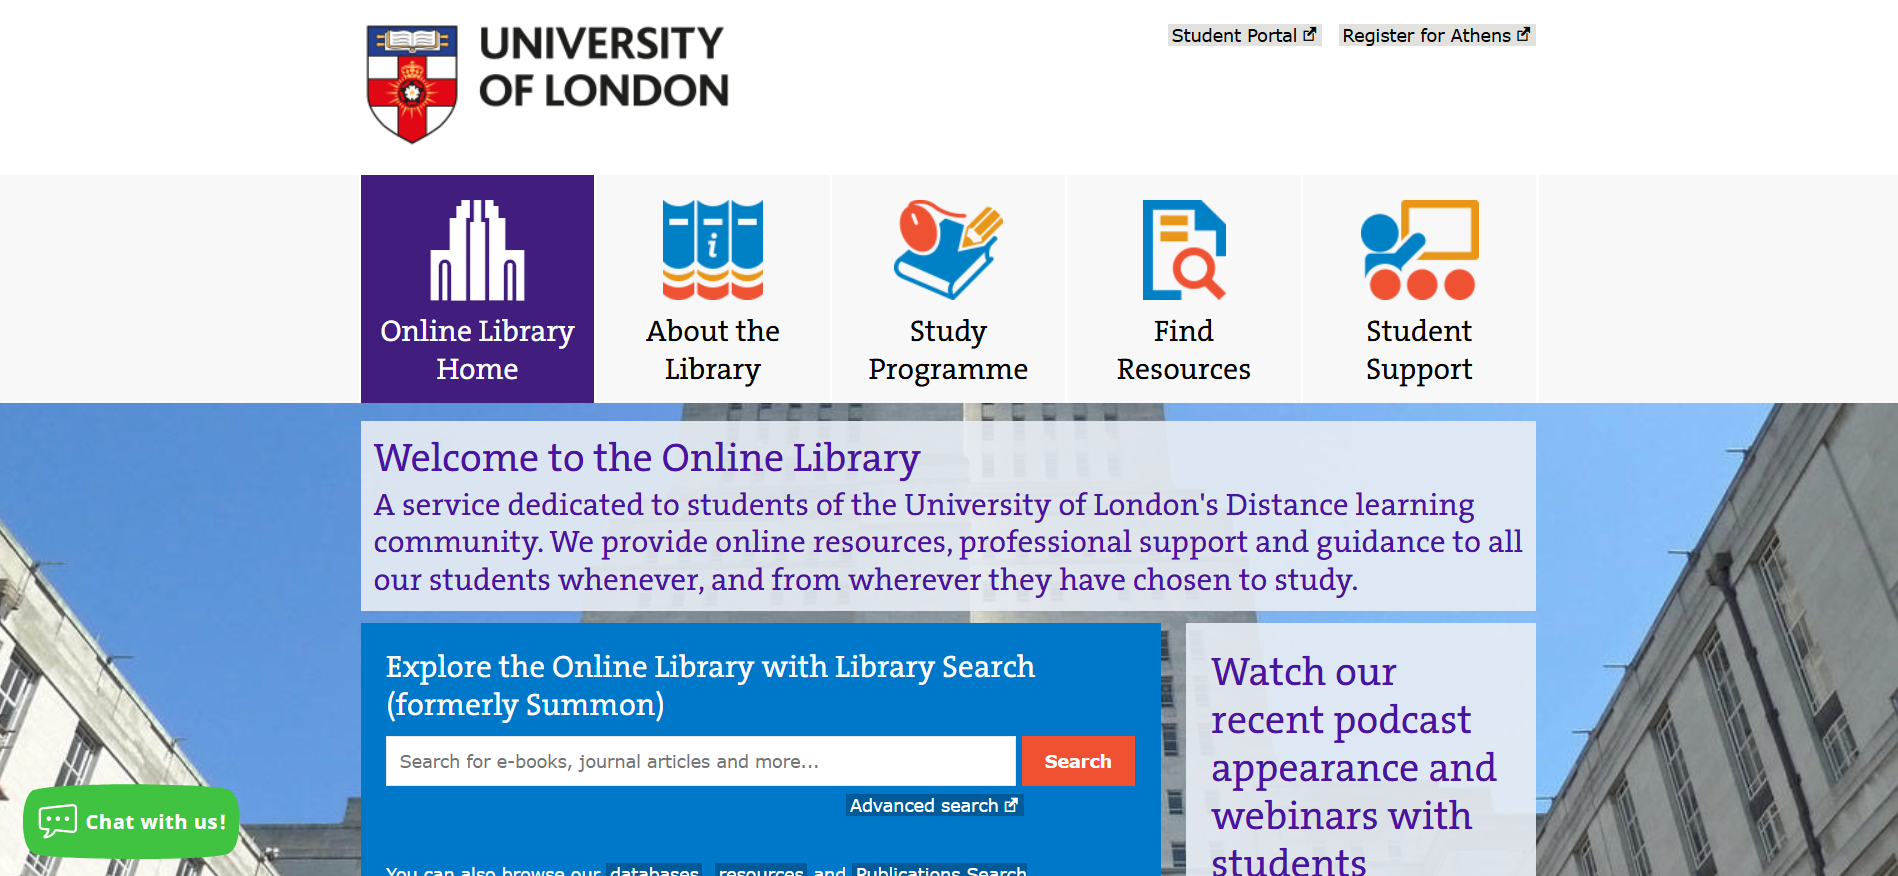
\includegraphics[width=0.8\linewidth]{Images/london_online_library_homepage.png} 
    \vspace{10pt}
    \caption{Giao diện tra cứu tập trung và công cụ hỗ trợ trực tuyến tại The Online Library - UoL}
    \label{fig:london_lib_homepage}
\end{figure}

Việc phân tích hệ thống UoL mang lại góc nhìn quan trọng về cách tối ưu hóa trải nghiệm trên môi trường số, đồng thời cũng bộc lộ những khoảng trống công nghệ khi chưa ứng dụng sâu các thuật toán thông minh vào quá trình tương tác.

\subsubsection{Điểm mạnh}
\begin{itemize}
    \item Cung cấp một điểm truy cập duy nhất cho toàn bộ tài nguyên số giúp tối ưu hóa thời gian tra cứu.
    \item Sử dụng giao thức xác thực hiện đại (OpenAthens) giúp bạn đọc dễ dàng truy cập từ xa mà không cần VPN.
    \item Tổ chức nội dung và tài liệu số theo từng chuyên ngành cụ thể giúp định hướng người dùng hiệu quả.
\end{itemize}

\subsubsection{Điểm yếu}
\begin{itemize}
    \item Mô hình chỉ giới hạn ở tài nguyên số, hoàn toàn bỏ qua các nghiệp vụ lưu thông và quản lý kho sách vật lý.
    \item Phương thức tra cứu tập trung dễ gây quá tải thông tin và thiếu thuật toán phân tích hành vi để gợi ý cá nhân hóa.
    \item Tính năng Chatbot hỗ trợ chỉ vận hành theo kịch bản tĩnh, chưa hiểu các truy vấn phức tạp và phụ thuộc vào thủ thư.
\end{itemize}

\subsection{Hệ thống Thư viện Đại học Delaware (UD Library)}

Hệ thống Thư viện Đại học Delaware (UD Library) tại địa chỉ \url{https://library.udel.edu/} đại diện cho mô hình quản trị thư viện đại học đa chi nhánh (Multi-branch University Library) có mức độ chuyển đổi số cao. Khác với UoL chỉ thuần túy về tài nguyên số, hệ thống của UD phải giải quyết bài toán phức tạp hơn: quản lý, phân phối dữ liệu phân tán từ thư viện trung tâm đến các thư viện chuyên ngành, và đặc biệt là việc tiên phong tích hợp Trợ lý ảo AI vào quy trình hỗ trợ sinh viên.

Trái tim của hệ thống này là công cụ tra cứu trung tâm mang tên \textbf{DELCAT} (Unified Discovery Service), đóng vai trò như một cổng giao tiếp duy nhất giữa người dùng và hàng triệu bản ghi từ mọi định dạng khác nhau. Điểm đáng chú ý là UD Library đã bắt đầu triển khai các giải pháp AI giao tiếp bằng ngôn ngữ tự nhiên để song hành cùng hệ thống tra cứu truyền thống này.

\begin{figure}[H]
\centering
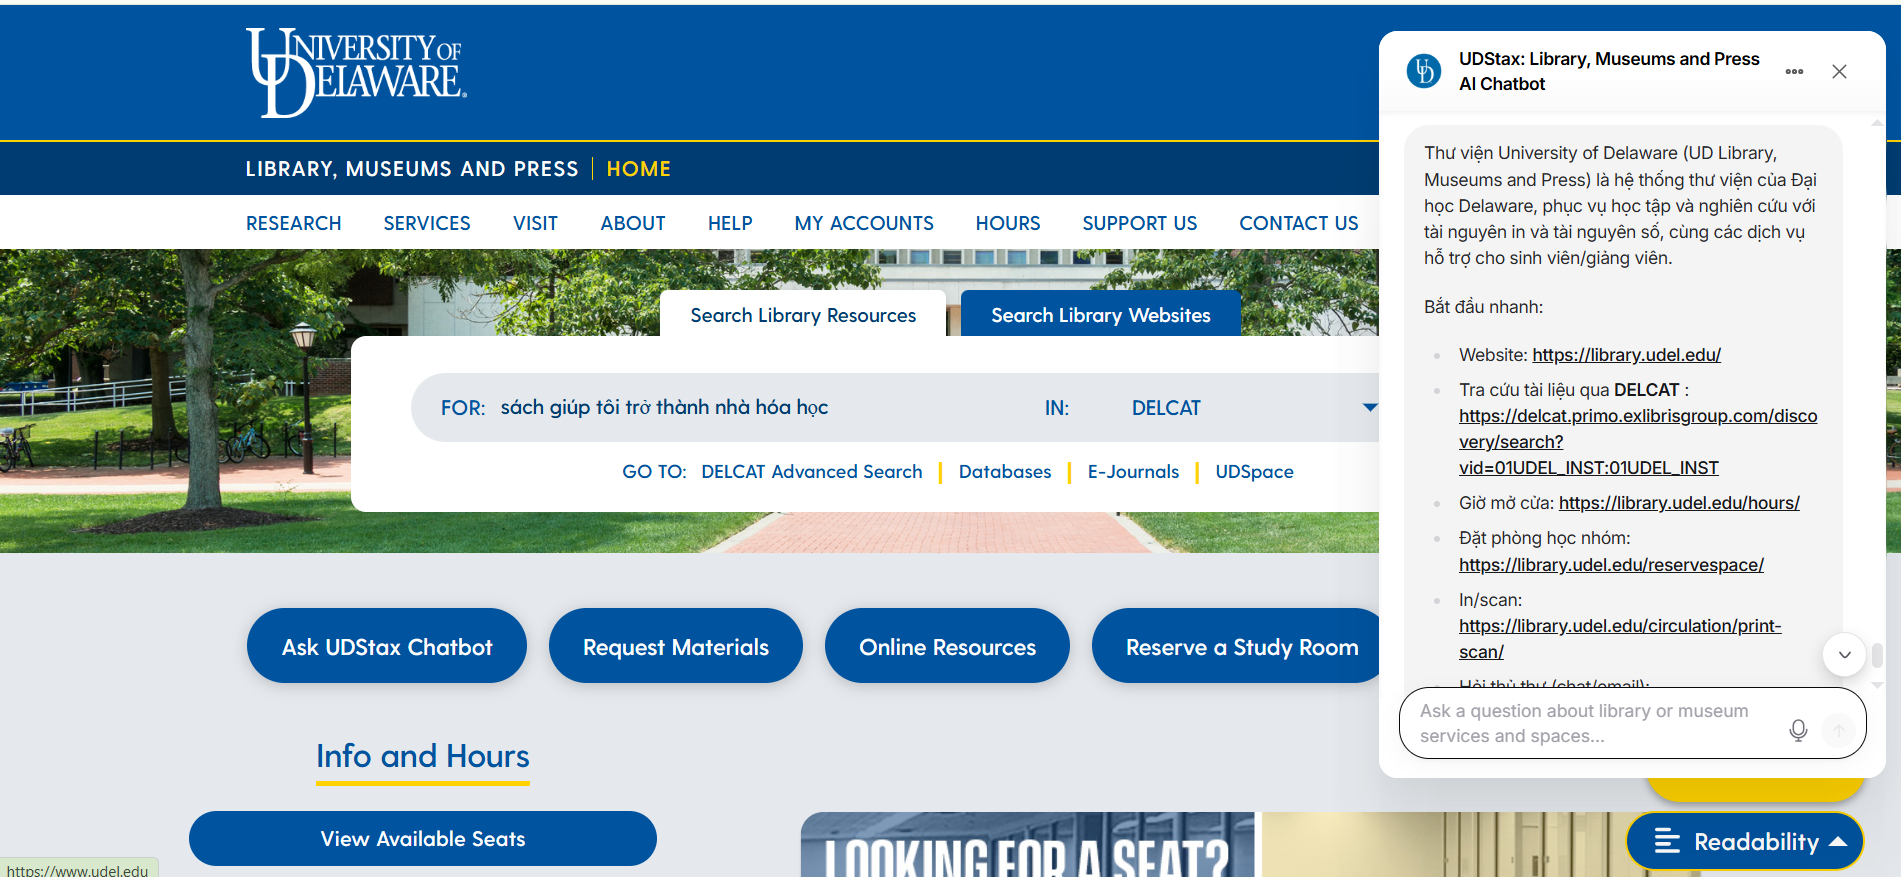
\includegraphics[width=0.8\linewidth]{Images/ud_library_homepage_chatbot.png} 
\vspace{10pt}
\caption{Giao diện dịch vụ khám phá hợp nhất DELCAT và công cụ AI hỗ trợ tại UD Library}
\label{fig:ud_delcat_search}
\end{figure}

Việc nghiên cứu UD Library cung cấp một góc nhìn quan trọng về cách xây dựng kiến trúc "Tất cả trong một" (All-in-one) và cách một trợ lý ảo AI đang được vận hành thực tế tại một trường đại học lớn.

\subsubsection{Điểm mạnh}
\begin{itemize}
\item Tích hợp trợ lý ảo có khả năng xử lý ngôn ngữ tự nhiên để tự động giải đáp các câu hỏi quy trình.
\item Hệ thống DELCAT hợp nhất việc tìm kiếm sách in và tài liệu điện tử trên cùng một giao diện duy nhất.
\item Kết nối trực tiếp các tiện ích phi truyền thống như đặt phòng học nhóm, in ấn và mượn liên thư viện.
\end{itemize}

\subsubsection{Điểm yếu}
\begin{itemize}
\item Chatbot hoạt động độc lập như kênh tư vấn thủ tục, chưa nhúng sâu vào lõi tìm kiếm để đề xuất sách trực tiếp.
\item Kiến trúc khám phá hợp nhất dễ gây ngợp thông tin cho bạn đọc khi trả về khối lượng kết quả quá lớn.
\end{itemize}


\subsection{Hệ thống Quản trị Thư viện Mã nguồn mở – Koha ILS}

Hệ thống Koha là phần mềm quản trị thư viện tích hợp (ILS) mã nguồn mở phổ biến nhất trên thế giới, được sử dụng rộng rãi tại nhiều trường đại học và thư viện công cộng. Khác với các cổng tra cứu OPAC hay nền tảng Discovery hướng tới người dùng cuối đã phân tích ở trên, Koha đại diện cho thế hệ hệ thống lõi (Backend) tập trung vào việc số hóa và giải quyết các bài toán nghiệp vụ phức tạp của người quản lý thư viện (Thủ thư).

Thông qua giao diện quản trị (Staff Client), Koha cung cấp các phân hệ đồ sộ để vận hành một thư viện vật lý và điện tử, bao gồm: Quản lý lưu thông (Circulation), Biên mục chuẩn quốc tế (Cataloging), Quản lý bạn đọc (Patrons), và Báo cáo thống kê (Reports). Việc nghiên cứu hệ thống Koha mang lại giá trị tham chiếu cực kỳ quan trọng trong việc thiết kế cấu trúc cơ sở dữ liệu và xây dựng các luồng quy tắc nghiệp vụ (Business Rules) cho khâu quản trị của đồ án.

\begin{figure}[H]
\centering
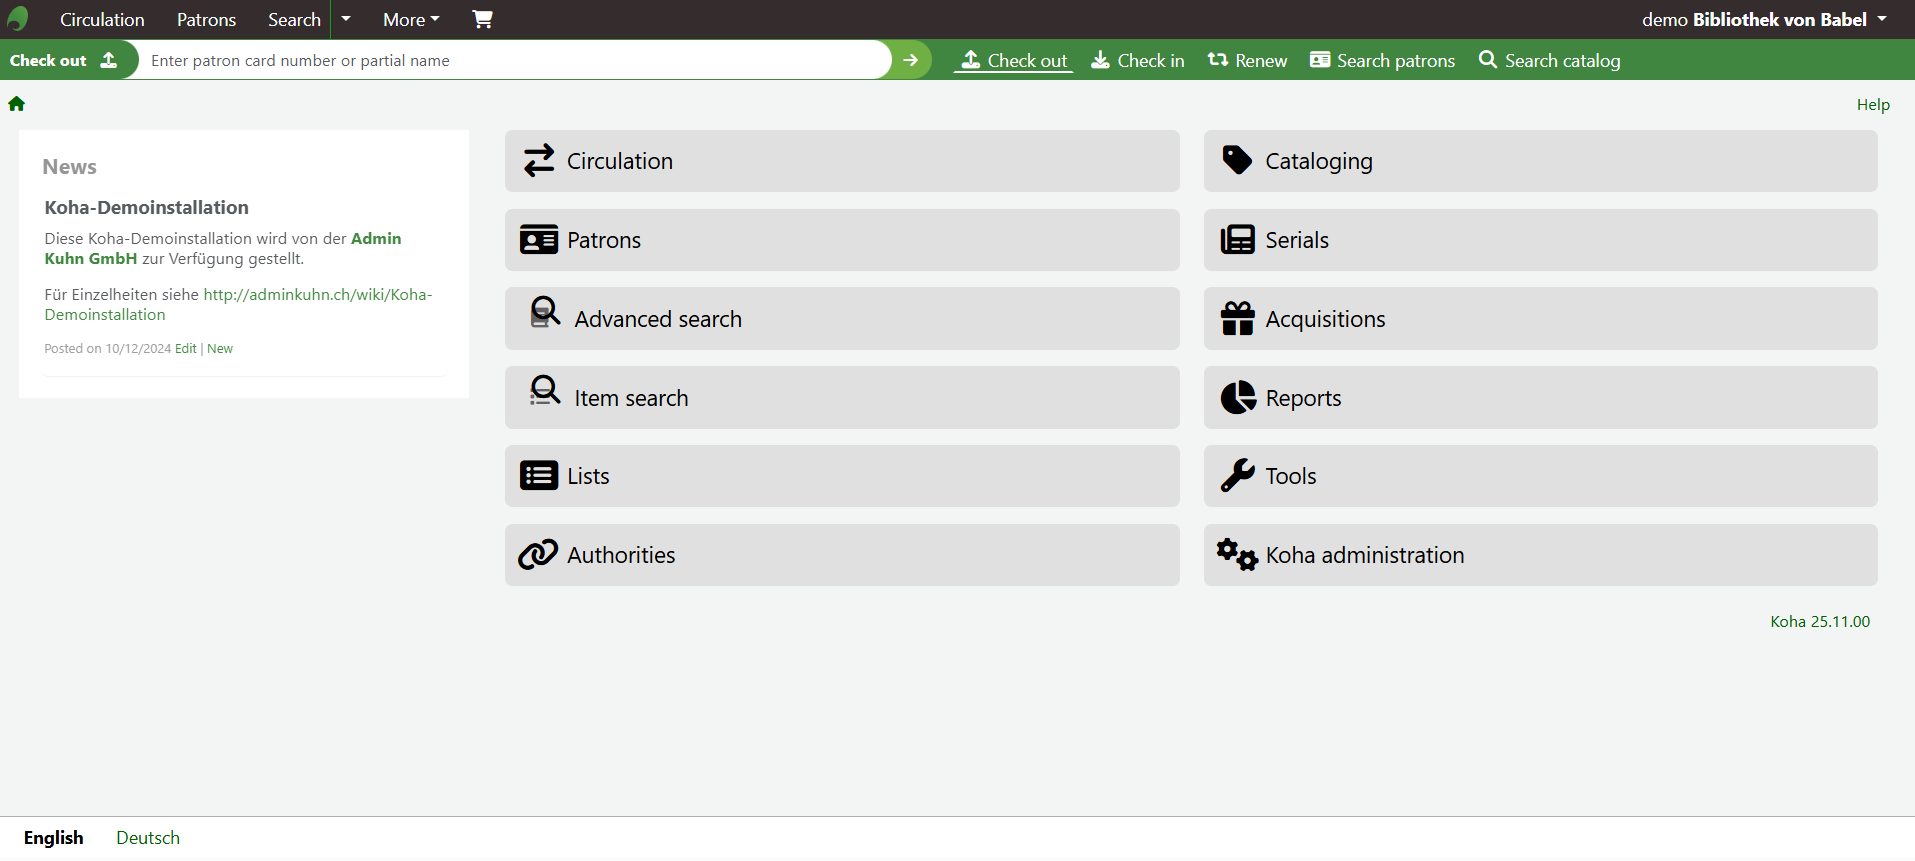
\includegraphics[width=0.8\linewidth]{Images/koha_staff_interface.png} 
\vspace{10pt}
\caption{Giao diện phân hệ quản trị (Staff Client) của hệ thống Koha}
\label{fig:koha_admin}
\end{figure}

Việc phân tích Koha giúp định hình rõ những tính năng cốt lõi bắt buộc phải có của một hệ thống quản lý thư viện, đồng thời bộc lộ những điểm nghẽn về mặt trải nghiệm người dùng mà phần mềm truyền thống đang gặp phải.

\subsubsection{Điểm mạnh}
\begin{itemize}
\item Hệ thống tuân thủ tuyệt đối các tiêu chuẩn dữ liệu thư viện quốc tế (như MARC21, Z39.50), đảm bảo tính nhất quán và khả năng liên thông dữ liệu chuẩn mực.
\item Phân hệ lưu thông (Circulation) cung cấp bộ quy tắc cực kỳ chi tiết, cho phép thiết lập ma trận luật mượn, trả, gia hạn và tính phí phạt theo từng nhóm đối tượng chuyên biệt.
\item Cung cấp hệ thống REST API tích hợp sẵn, cho phép các ứng dụng bên thứ ba dễ dàng giao tiếp và trích xuất dữ liệu khi cần mở rộng nền tảng.
\item Hệ thống báo cáo (Reports) hỗ trợ truy vấn trực tiếp bằng câu lệnh SQL, mang lại sự linh hoạt tối đa trong việc trích xuất số liệu quản trị.
\end{itemize}

\subsubsection{Điểm yếu}
\begin{itemize}
\item Giao diện quản trị (UI/UX) cồng kềnh, thiết kế theo hướng biểu mẫu truyền thống với quá nhiều trường thông tin dẫn đến thời gian đào tạo thủ thư (learning curve) kéo dài.
\item Luồng xử lý nghiệp vụ nhập liệu mang tính thủ công cao, thiếu vắng các cơ chế hỗ trợ phân loại hay trích xuất tự động thông minh.
\item Kiến trúc hệ thống mang tính nguyên khối (Monolithic), cấu trúc cơ sở dữ liệu phức tạp gây khó khăn cho việc bóc tách, tùy biến nhanh các chức năng đơn lẻ.
\end{itemize}